\subsubsection{UC5 - Login manuale}
\begin{figure}[h]
	\centering
	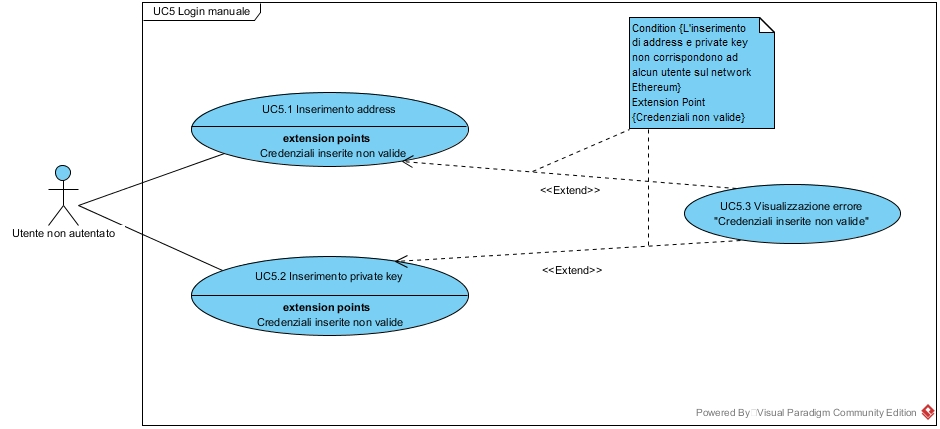
\includegraphics[width=0.8\linewidth]{res/img/UC5.jpg}
	\caption{Diagramma UC5 - Login manuale}
\end{figure}
\begin{itemize}
	\item \textbf{Attori primari:} Utente non autenticato;
	\item \textbf{Descrizione:} l'utente, mediante il comando "login" ha la possibilità di autenticarsi al network \textit{Ethereum\glo} inserendo manualmente da \textit{CLI\glo} la propria \textit{private key\glos} e password e, contestualmente, salvare in automatico le credenziali di accesso su un file sul proprio dispositivo;
	\item \textbf{Pre-condizioni:} l'utente ha visualizzato la guida introduttiva e desidera autenticarsi manualmente;
	\item \textbf{Post-condizioni:} il sistema avrà autenticato o meno l'utente a seconda dei valori di accesso inseriti dalla \textit{CLI\glos};
	\item \textbf{Scenario principale:}
	\begin{enumerate}
		\item L'utente scriverà un comando da \textit{CLI\glos}, composto nel seguente modo:
		\begin{itemize}
			\item nome del comando "login";
			\item \textit{private key\glos};
			\item password
		\end{itemize}
		\item Verrà visualizzato a schermo un messaggio relativo all'esito dell'autenticazione;
		\item Sarà salvato un file sul dispositivo contenente le credenziali di accesso.
	\end{enumerate}
	\item \textbf{Estensioni:} 
	\begin{itemize}
		\item \textbf{UC22}: errore di autenticazione dovuto all'inserimento errato di \textit{private key\glos}/password non corrispondenti ad alcun account \textit{Ethereum\glos}.
	\end{itemize}
\end{itemize}
